\documentclass[ICS, PP, english, final]{ICS_thesis}
\graphicspath{{pics/}{logos/}}


%_________MACROS_________ (optional and customizable - see output)
%% include packages for your work in here
% \usepackage[colorinlistoftodos]{todonotes}        % for handling TODOs
\usepackage{setspace}
\usepackage{acronym}
\usepackage{listings}
\usepackage{xcolor}

% using the todonotes package in some nice ways (see packages.tex)
\newcommand{\add}[2][]{\todo[color=blue!40,#1]{#2}{}}
\newcommand\optional[2][]{\todo[inline, color=cyan!40, caption={2do},
	#1]{\begin{minipage}{\textwidth-4pt}#2\end{minipage}}{}}

% math macros
\newcommand{\set}[1]{\boldsymbol{#1}}
\renewcommand{\vec}[1]{\mathbf{#1}}

% % commands for easy referencing
\newcommand{\fref}[1]{Figure~\ref{#1}}
\newcommand{\tref}[1]{Table~\ref{#1}}
\newcommand{\eref}[1]{Equation~\ref{#1}}
\newcommand{\cref}[1]{Chapter~\ref{#1}}
\newcommand{\sref}[1]{Section~\ref{#1}}
\newcommand{\aref}[1]{Appendix~\ref{#1}}

% fancy source code listings: http://stackoverflow.com/questions/741985/latex-source-code-listing-like-in-professional-books
% usage: \lstinputlisting[label=samplecode,caption=A sample]{sourceCode/HelloWorld.java}
\definecolor{light-gray}{gray}{0.95}
\usepackage{listings}
\usepackage{courier}
\lstset{
         basicstyle=\footnotesize\ttfamily, % Standardschrift
         numbers=left,               % Ort der Zeilennummern
         numberstyle=\tiny,          % Stil der Zeilennummern
         stepnumber=0,               % Abstand zwischen den Zeilennummern
         numbersep=5pt,              % Abstand der Nummern zum Text
         tabsize=2,                  % Groesse von Tabs
         extendedchars=true,         %
         breaklines=true,            % Zeilen werden Umgebrochen
         keywordstyle=\color{red},
         stringstyle=\color{white}\ttfamily, % Farbe der String
         showspaces=false,           % Leerzeichen anzeigen ?
         showtabs=false,             % Tabs anzeigen ?
         xleftmargin=0pt,
         framexleftmargin=10pt,
         framexrightmargin=10pt,
         framexbottommargin=0pt,
         backgroundcolor=\color{light-gray},
         showstringspaces=false      % Leerzeichen in Strings anzeigen ?
}

\lstdefinestyle{customc}{
  	belowcaptionskip=1\baselineskip,
  	breaklines=true,
  	%frame=L,
  	language=BASH,
  	showstringspaces=false,
 	basicstyle=\footnotesize\ttfamily\color{blue!40!black},
 	keywordstyle=\bfseries\color{green!40!black},
  	commentstyle=\itshape\color{purple!40!black},
  	%identifierstyle=\color{blue}, %color of actual code
 	stringstyle=\color{orange},
    numbers=left,               % Ort der Zeilennummern
    numberstyle=\tiny,          % Stil der Zeilennummern
    stepnumber=2,               % Abstand zwischen den Zeilennummern
    numbersep=5pt,              % Abstand der Nummern zum Text
    tabsize=2,                  % Groesse von Tabs
    extendedchars=true,         %
    showspaces=false,           % Leerzeichen anzeigen ?
    showtabs=false,             % Tabs anzeigen ?
  	xleftmargin=\parindent,
    framexleftmargin=10pt,
    framexrightmargin=10pt,
    framexbottommargin=0pt,
    backgroundcolor=\color{light-gray},
}

\lstset{style=customc}% i have deleted "escapechar=@,"

%_______Start_Document______________________________________
\begin{document}


\title{RoboCup SS17}

\student{B.Sc. Tianming Qiu} 			%% your name
\yearofbirth{30.03.1993}	                	%% date of birth
\street{Felsennelkenanger 15}			%% your address
\city{80937, Munich}						%		"
\phone{+49 17643387325}					%% your telephone-no.
\supervisor{Mohsen Kaboli}				%% your supervisor
\start{24.04.2017}						%% start date
\finalrep{24.07.2017}					   	%% final presentation / date

\maketitle



% ________Abstract__________________________________________-
\topmargin5mm
\textheight220mm
\pagenumbering{arabic}
\phantom{u}
\begin{abstract}
RoboCup is a competition for soccer robot held annually and we work on the RoboCup Standard Platform League (SPL) by using humanoid robot NAO, based on the code framework from University of Bremen's team B-Human.

Self-localization is a very important task for NAOs during the match. The action decisions, ball tracking and different team cooperation strategies are dependent on the precise location on the standard soccer field. Self-localization is also related to computer vision and statistical signal processing. These topics are the foundations of autonomous robot. So this semester I focus on figuring it out, how does NAO localize itself on the soccer field by cameras and how could it be improved.

The current method in B-Human framework has been continuously developed, verified and implemented for several years. It has been considered as state-of-the-art method which is already very robust and compact. The main idea of self-localization in B-Human framework is to apply particle filter with unscented Kalman filter for each particle to estimate robot pose. But there are still some issues that when robot is walking, some shaking noises from camera will cause deviations in visual odometry. PnP pose estimate would be adopted instead of relative distance calculation, which would take all the transforms generally into consideration and eliminate the error.
\end{abstract}

% %%%%%%%%%%%%%%%%%%%%% Widmung %%%%%%%%%%%%%%%%%%%%%%%%%%%%%%%%
\phantom{u}
\phantom{1}\vspace{6cm}
\begin{center}
%Hier die Widmung oder leer lassen
\end{center}


\pagestyle{fancy}

%%%%%%%%%%%%%%%%%%%Inhaltsverzeichnis%%%%%%%%%%%%%%%%%%%%%%%%%%
\tableofcontents

%%%%%%%%%%%%%%%%%%%%%%%%%%%%%%%
% ACTUAL CONTENT OF YOUR WORK %
%%%%%%%%%%%%%%%%%%%%%%%%%%%%%%%
%%%%%%%%%%%% Kapitel - externe Dateien zur Ordnung%%%%%%%%%%%%%
\chapter{Introduction}
RoboCup is a competition for soccer robot held annually, which aims at promoting researches on robot and artificial intelligence. We work on the RoboCup Standard Platform League (SPL) by using humanoid robot NAO. There are 5 players for each side: goalkeeper, defender, supporter and striker. Different roles share some same functions such as self-localization, tracking the ball, kicking and so on. They also have different strategies according their distribution on the field just like the real soccer match. Of course the necessary communication and coorperation are required to achieve better performance in the match. One of the most successful team is B-Human from University of Bremen. They have won the championship five times. Last year TU Munich also set up our own RoboCup team called ``TUM Lion".
\section{Motivation}
The course ``Introduction Lab Humanoid RoboCup" in this semester is given for the students are interested in RoboCup and gives them a brief idea about RoboCup and the general knowledge of practice on autonomous robot loacalization, computer vision, motion control and multi-robot cooperation tasks. This semeater's project is based on the code framework from University of Bremen's team B-Human. With the help of the open source framework could let us start the project more quickly and do some specific reasearch on the topic what we are interested in or more familiar with. At the same time, some issues will be found and could be improved or considered as another new strategy.

\section{My Work}
Since we have already get the access to the state-of-the-art open source framework, so the first stage is to get familiar with the procedure of NAO operating and the codes. It includes:
\begin{itemize}
   	\item Basic operation on NAO and remote control through SimRobot
   	\item Calibration
	\item Understand how the current framework realize the self-localization
\end{itemize}

The second stage is focusing on self-localization and finding some interesting part to improve. Firstly I learned the Markov localization theory of mobile robot such as particle filter and unscented Kalman filter, which is used in the B-Human framework. Then the PnP pose estimation method is adopted to elimanate the current visual odometry error. In Chapter 2 I will introduce how does the current method figure out the localization of robot and the procedure of particle filer and unscented Kalman filter. In Chapter 3 I will show the visual odometry procedure of B-Human and explain what kind of noise it could be as well as the method that I applied.

\chapter{Self-Localization}\label{Chap:PF}
This chapter introduces the concrete method used in the current framework for NAO, the mobile roboter lacalization. RoboCup self-localization is a problem that NAO robot could determine its pose, which includes both position and angular, relative to the given map of the standard soccer field. Almost all the tasks for each robot player require knowledge of its pose on the field. We call this problem as rather a self-localization than a SLAM(Simultaneous localization and mapping) problem, one important reason is the map of the environment has been provided as prior knowledges. Self-localization could be treated as a problem of coordinate transformation. Map of the field or environment is described as the global coordinate system, which does not rely on robot's pose. The robot pose will be finally transformed into the global frame and represented as a global coordiante\cite{thrun2005probabilistic}. In our project the NAO pose is only changes in a plane, the $z$ element is always remains as zero since the robot always stands firmly on the ground. So the pose could be written as $(x,y,\theta)^T$.

However, the pose of robot could not be aquired directly, instead it could be inferred from the sensor data, which here come from camera. The sensor could not be hundred percentage accurate, it alway contains noise, especially image processing by using camera. So we have to find a proper method to calculate the pose from imperfect sensor data, which will be introduced in this chapter.

\section{General Framework: Particle Filter}
For self-localization, B-Human uses a particle filter based on the Monte Carlo method \cite{fox1999monte} as it is a proven approach to provide accurate results in such an environment \cite{rofer2005particle}. The reason for selecting particle filter in this self-localization problem is that in the RoboCup soccer match the robot will from time to time fall down, and then it will not get the correct knowledge of its position. The problem is that the robot might believe it knows where it is while it does not. This is called kidnapped robot problem \cite{thrun2005probabilistic}. So the particle filter will be adopted to solve this kidnapped robot problem and it does not demand initial position of robot.

The particle filter is a kind of bayes filter, based on Monte Carlo method. It uses several samples as particles to describe the posterior. In particle filter, the samples of a posterior distribution are called particles are represented as \cite{thrun2005probabilistic}: 
\[
\mathcal{X}_t:=x_t^{[1]},x_t^{[2]} \dots x_t^{[M]}
\]
The posterior of each particle $x_t^{m} (with 1 \leq m \leq M)$ is the probalbilty of the state at specigic time $t$. Usually, M, the number of the particles is very large to get a as perfect as possible approxiamtion, since particle filter is a non-parametrical method to estimate the state updating. However in the RoboCup situation, only 12 to 16 particles are adopted. Because the memory space and computaion speed are both limited on the robot NAO. During the match, it has a high demanding on instantaneity. Here I have not tested or verified the effectiveness of the so small number of samples. But in recent years B-Human team even drop the particles from 16 to 12 \cite{BHumanCodeRelease2010} and it is proven in practice which shows a great robustness and outstanding performance. Then how does robot NAO apply particle filter to localize itself is shown in the flowchart \fref{Ffc.sub.1}.
\begin{figure}[tbp]
\centering
\subfigure[Particle filter]{
\label{Ffc.sub.1}
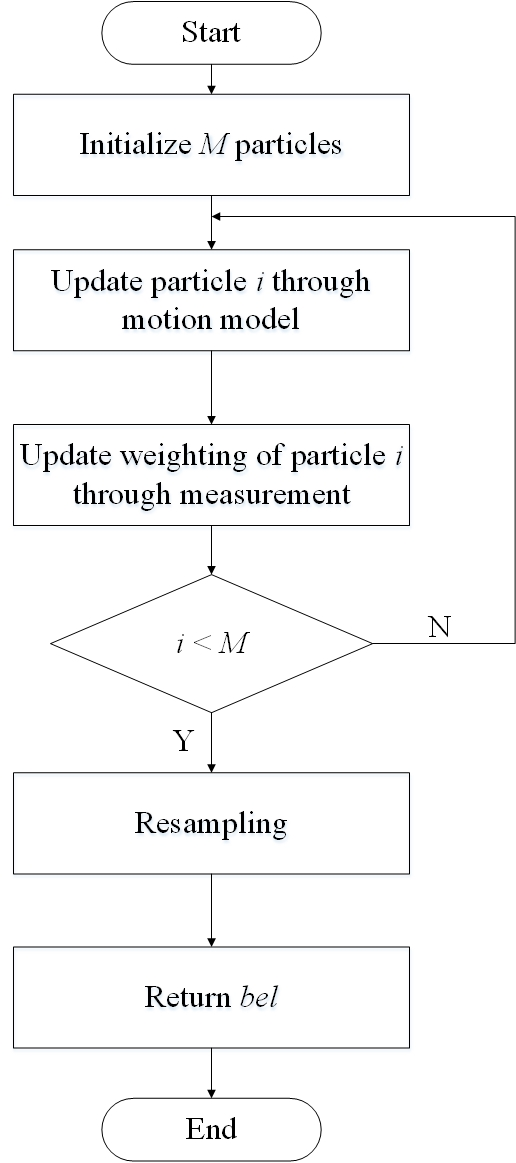
\includegraphics[width=0.3\textwidth]{pics/PF.jpg}}
\subfigure[combine PF and UKF]{
\label{Ffc.sub.2}
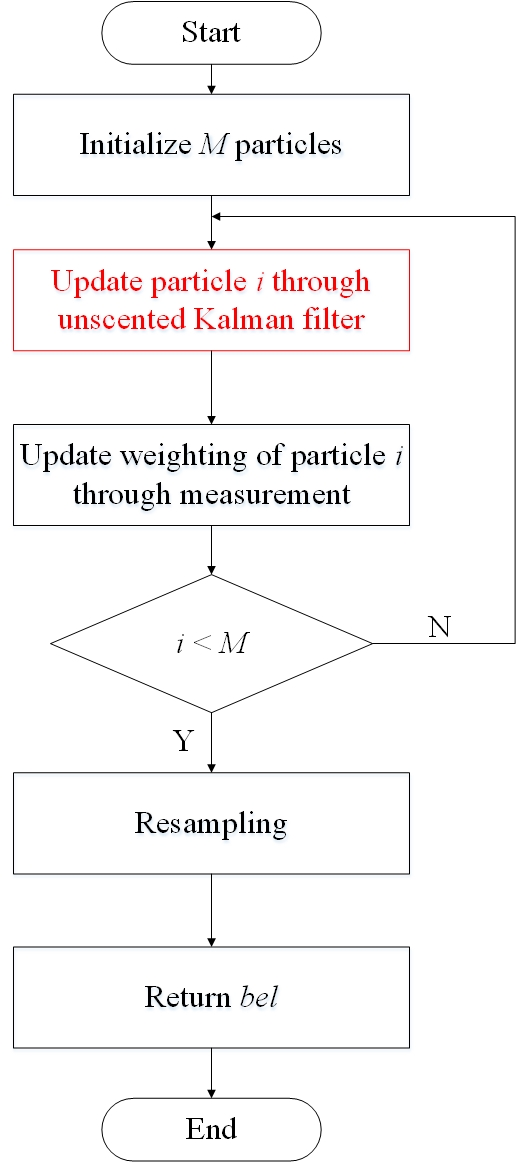
\includegraphics[width=0.3\textwidth]{pics/cpf.jpg}}
\caption{Self-localization based on particle filter flowchart}
\label{ffc}
\end{figure}

\section{Combination with Unscented Kalman Filter}
Since 2012, B-Human framework made a big change on self-localization: a combination of a particle filter and an Unscented Kalman filter is used.
The former computes a global position estimate; the latter performs local tracking for refining the global estimate \cite{BHumanCodeRelease2012}. 
This implementation will improve the local accuracy of particle filter and further results in improvement of localization precision. The change has shown in the \fref{Ffc.sub.2}. 

The idea behind the Unscented Kalman filter is similar to the original Kalman filter. However it is applied for the non-linear motion model and provides priciser result than Extented Kalman filter which uses first order approximation of Talor seires. It generates sigma points and uses the unscented transform to describe the non-linearity. The mean as well as covariance of states will also be modified with measurement and finally be returned. 

Generally, the localization process will use particle filter to estimate the robot pose and each particle will use unscented Kalman filter to update the pose of the sample.

\chapter{Improvement of Visual Odometry}\label{Chap:Imp}
Above the procedure of self-localization was described in general. Particle filter require sensor measurement to calculate the weighting for each particle and Unscented Kalman filter demands the sensor measurements to update the motion predictions. Visual odometry is a widely used with strong functions sensor measurement method, which is applied in this situation and provides the measurement for each kind of filter. So the accuracy of pose estimated by visual part will definitely have an obvious influence on the final result. This chapter will introduce what knowledge of the sensor measurement can provide and how the sensor measurement take place. 
\section{The current method}
\subsection{Visual odometry procedure}
There are several sensors to acquire information from the environment on NAO: camera, microphone and sonar. From them only the camera is adopted, since the environment of the soccer match will be quite complicated, for example:
\begin{itemize}
    \item The white border lines and green field are on the same plane.
    \item The goal posts are perhaps too far away from the robots sometimes.
    \item There are 6 moving robots on the field, which the opponents are distinguished from our teammates only by colors.
    \item The ball is small and the detection of a ball requires high precision.
\end{itemize}
So based on above reasons, the another sensors are not qualified for the requirements. However, the camera is suitable for each specific task and the computer vision skill as well as visual odometry are being perfect so far.

There two cameras on the NAO's head which can provide large FOV. Several tasks such as image preprocessing, feature detection(including: line perception, penalty mark perception, ball perception) and data association will be performed on the image gathered by each camera. B-Human's current vision system provides a variety of perceptions that have all been integrated into the sensor model: goal posts (ambiguous as well as unambiguous ones), line segments (of which only the endpoints are matched to the field model), line crossings (of three different types: L, T, and X ), and the center circle \cite{BHumanCodeRelease2012}. These features can be associated to the feature detected in pixel images. The detailed of these tasks will not be mentioned in my part of report, which are introduced by my teammates. My work is that suppose the the feature detection and data association have been finished.

Based on feature detection and data association, the corresponding point pairs have been already found. For example the goal post in figure i. whose coordinate in the homogeneous global 3D world could be represented as $(X,Y,0,1)^T$. And the corresponding homogeneous coordinate in pixel coordinate can be written as $(x,y,1)^T$. Since the camera calibration matrix, including both intrinsic and extrinsic calibration parameters, has been acquired through camera calibration before each match. Assuming the camera model as pinhole camera model shown in \fref{fig: camera} \cite{hartley2003multiple}: 
\[ % without number
\mathbf{x} = \mathbf{K} \cdot \mathbf{X}_{cam}
\]
\begin{figure}[!htb]
    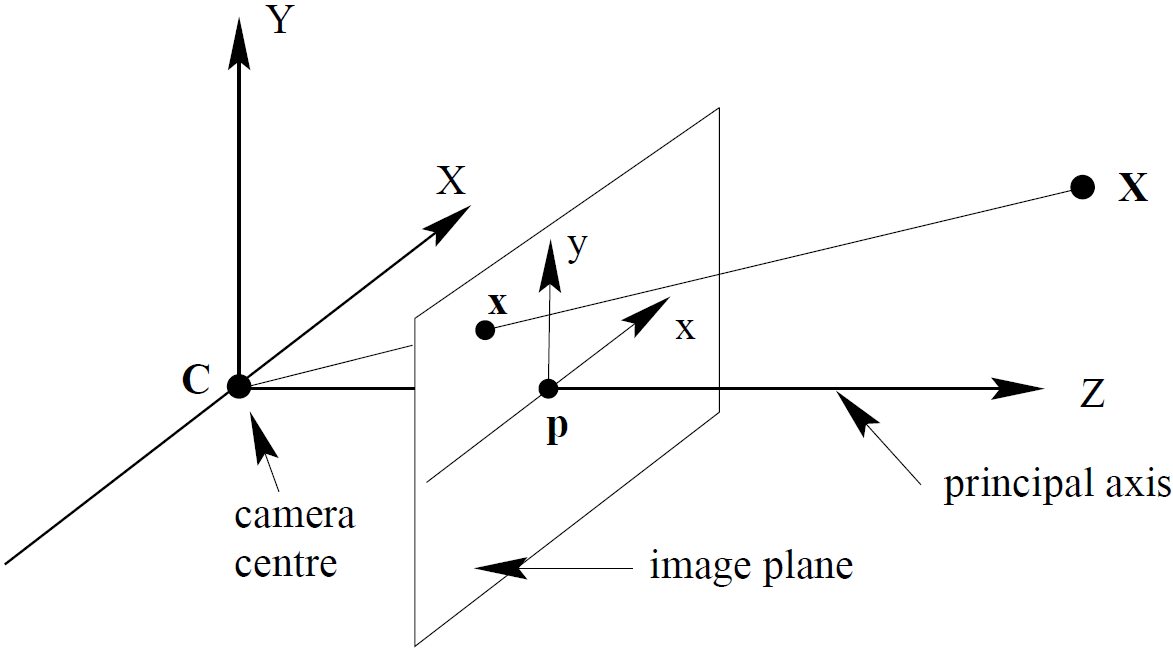
\includegraphics[width=0.4\textwidth]{pics/cameramodel.png}
    \centering
    \caption{Pinhole camera model}
    \label{fig: camera}
\end{figure}

So we could get the corresponding 3D goal post coordinate in the ideal camera frame. Since we know the geometrical value of NAO's body construction, we can transform the coordinates into the robot frame, which is shown in the \fref{fig: trans.sub.1}
\begin{figure}[tbp]
\centering
\subfigure[Coordinate transform]{
\label{trans.sub.1}
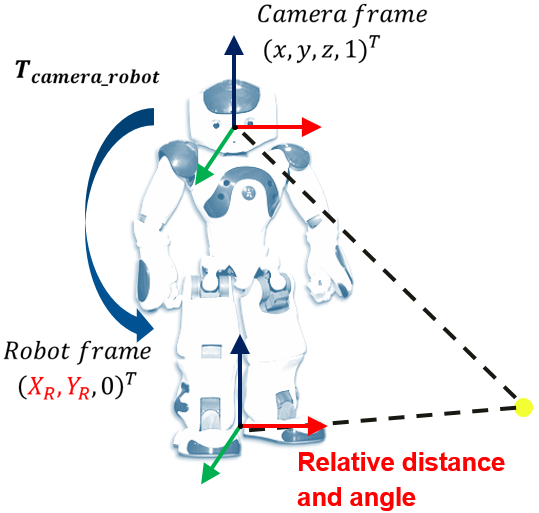
\includegraphics[width=0.45\textwidth]{pics/coordinate_transform.png}}
\subfigure[Relative pose to landmark]{
\label{trans.sub.2}
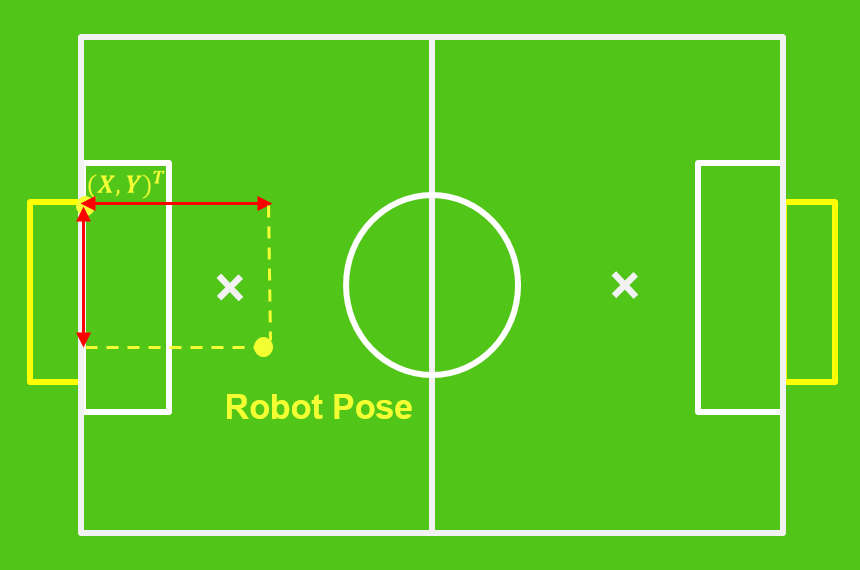
\includegraphics[width=0.45\textwidth]{pics/relative.png}}
\caption{Pose estimation}
\label{fig: trans}
\end{figure}
Based on this, we could get the related distance between robot and the goal post in robot frame. At the same time, the precise location of goal post in the global field is also known. So we could calculate the robot pose from this above information.
\subsection{Current problem}
In the process of transforming the coordinate from camera frame into robot frame, the current method only use a constant transform. However when robot is walking, it cannot always be extremely vertical to the ground. The central line of its body and camera on the head will have an arbitrary angle of tilt. Also due to detecting of the environment, robot always turn around its head or even look up and down, but this information will also create bias by coordinate transforming. Then it will cause a bias on the camera frame transform, which is shown in \fref{fig: error}. This error between the real robot base coordinate and the result calculated by the constant transform will further affect the pose estimation. 
\begin{figure}[!htb]
    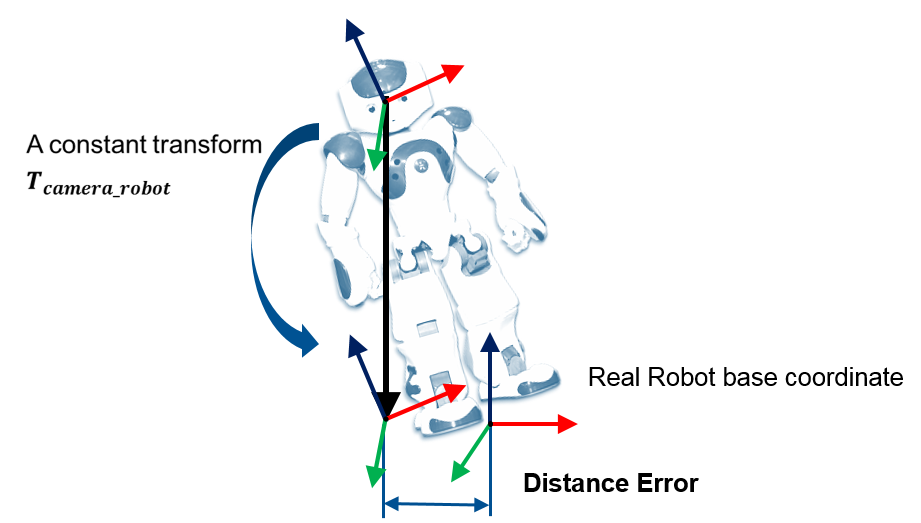
\includegraphics[width=0.7\textwidth]{pics/error.png}
    \centering
    \caption{Position error by a constant transform}
    \label{fig: error}
\end{figure}\\

\section{PnP Pose estimation}
Since the current method contains the tilting and shaking error so I apply the PnP method \cite{ETHPnP} which could eliminate the error by consider the transform in a more direct way. Reconsidering corresponding point pair $\mathbf{x}:=(x,y,1)^T$ in pixel coordinate and $\mathbf{X}:=(X,Y,0,1)^T$ in 3D global space. They should have this following relationship \eqref{relation}:
\begin{equation}
\mathbf{x} = \mathbf{T}_{image2field} \cdot \mathbf{X}_{field} \label{relation}
\end{equation}
And the transform matrix $\mathbf{T}_{image2field}$ could be represented as three parts: 
\begin{equation}
\mathbf{T}_{image2field}=\mathbf{K} \cdot \mathbf{T}_{camera2robot} \cdot \mathbf{T}_{robot2field} \label{transform}
\end{equation}
In \eqref{transform} what we can figure out from the corresponding point pairs is $\mathbf{T}_{image2field}$, and what we want to know is $\mathbf{T}_{robot2field}$. If we know the $\mathbf{T}_{robot2field}$ then we could directly read robot pose from this matrix. Also, the camera calibration matrix $\mathbf{K}$ is also already known because the calibration has been done before each match. 
$\mathbf{T}_{robot2field}$ can also be represented as \eqref{Trf}:
\begin{equation}\mathbf{T}_{robot2field}=
\begin{bmatrix}
\mathbf{R} & \mathbf{T}
\end{bmatrix}=
\begin{bmatrix}
cos\alpha & sin\alpha & 0 & T_x\\
-sin\alpha & cos\alpha & 0 & T_y\\
0 & 0 & 1 & 0
\end{bmatrix} \label{Trf}
\end{equation}

There are 4 unknown parameters in \eqref{Trf}, so at least 2 pairs of corresponding points are required to solve the equation. The 2 pairs of corresponding points can be selected by two goal posts or the start and end point of a specific line. Suppose $\mathbf{M}:=\mathbf{K} \cdot \mathbf{T}_{camera2robot}$, elements in $\mathbf{M}$ are all known values, so the equation can be written as \eqref{Trf2}:
\begin{equation}\mathbf{x}=\mathbf{M} \cdot
\begin{bmatrix}
\mathbf{R} & \mathbf{T}
\end{bmatrix} \cdot \mathbf{X} =\mathbf{A}\cdot \mathbf{X}
\label{Trf2}
\end{equation}

\begin{equation}[\mathbf{x_1} \quad \mathbf{x_2}]=
\mathbf{A}\cdot [\mathbf{X_2} \quad \mathbf{X_2}]
\label{Trf3}
\end{equation}

So, in \eqref{Trf3} it shows the how does two pairs of corresponding points calculate matrix $\mathbf{A}$ which contains four unknown parameters. If we have more than 4 pairs of corresponding points, SVD method for minimum solution finding could be applied.






\chapter{Conclusion}
\section{Result and Comparison}
Before the robot always gets lost and cannot go to the assigned area, such as defending area for defender even at the begining of match. After using PnP pose estimation method, the accuracy of pose calculation has been improved. The self-localization process is much more quick and robost. Averagely, the robot NAO could go to the specific position from initial position out of the border in 30 seconds. 
The current method which based on only one pair of cooresponding points will be less computation cost but it does not consider the tilting pose of the robot body and rotating of the robot head as well as its camera. However the precise localization of robot is more important and the result will be fed to both unscented Kalman filters and particle filter, which will further affect the self-localization.
\section{Future Work}
\subsection{Come up with a more adequate noise model}
This semester we focused on the visual odometry part, just the sensor measurement of the both two filter method. The motion model also plays an important role on the localization and is restricted with noise comes from actuators of each joint as well as the ground friction at the same time. So in the future, this part of work should be done and set up a more proper and sceintifc noise model to describe the uncertainty of motion model.

\subsection{Search for ball}
There is still some problem of searching for the ball, this part belongs not to the localization problem, but a tracking problem. 

\subsection{Data asscocaition error}
According to the both cuurent method and PnP pose estimation method, the correctness of data association determines the final quality of self-localization directly. Wheather the current data asscociation robust enough and which noise comes from, these issues should be more discussed.

\subsection{Communication with another robots}
This semster we only operate on each single robot without communication with another team players. The communication is very useful and it can gather more information and more fast. For example, if one of the robot has seen the ball, it could `tell' other robot where the ball is. Then the other robot will not implement the ball search task any more and do another more efficeint job. Furthermore, if two robot detect the ball at the same time, they could make a data fusion through communication to improve the accuracy.



% \appendix
% 	\input{./chapters/Appendix.tex}

%%%%%%%%%%%%%%%%%%Acknoledgments %%%%%%%%%%%%%%%%%%%%%%
\cleardoublepage
\chapter*{Acknowledgments}
\markright{ACKNOWLEDGMENTS}
First of all, I would like to express my thanks to Prof. Dr. Gordon Cheng and Chair of Cognitive Systems for offering this course and all the hardware equipments.

I would further like to thank our supervisor Mohsen Kaboli for your patient help and many constructive suggestions. You are always willing to share your experiences and give us significant guides. Your office is always open to us. You are strict to us but I really learn a lot from that. Not only the experiment itself also the way how to deliver a presentation.

Also, I would appreciate the help offered by our teaching assistant Zhiliang Wu, who prepared all the lab stuff for us and wrote detailed tutorials that let me know how to operate NAO step by step. Your careful work makes me to get start quickly as soon as possible and gives me a lot confidence to finish the task. 

I am particularly thankful to my team mate: Yao, Fabian, Zhiyi, Jingjie, and Minkai. We discussed a lot and you always give me supports.

%%%%%%%%%%%%%%%%%%_Abbildungsverzeichnis %%%%%%%%%%%%%%%%%%%%%%
\cleardoublepage
\addcontentsline{toc}{chapter}{List of Figures}
\listoffigures

% %%%%%%%%%%%%%%%%%%_Acronyms and Notations %%%%%%%%%%%%%%%%%%%%%%
 %\cleardoublepage
% \chapter*{Acronyms and Notations}
% %%%%%%%%%%%%%% ACRONYMS %%%%%%%%%%%%%%%%%
\begin{acronym}
	\acro{HRC}{Human-Robot Collaboration}
	\acro{HRI}{Human-Robot Interaction}
	\acro{HRT}{Human-Robot Team}	
\end{acronym}

%%%%%%%%%%%%%%%%%%Literaturverzeichnis %%%%%%%%%%%%%%%%%%%%%%%%
\cleardoublepage
\addcontentsline{toc}{chapter}{Bibliography}
\bibliography{mybib}
\bibliographystyle{unsrt}

%%%%%%%%%%%%%%%%%%%%License %%%%%%%%%%%%%%%%%%%%%%%%%%%%%%%%%%%
%\cleardoublepage
%\chapter*{License}
%\markright{LICENSE}
%This work is licensed under the Creative Commons Attribution 3.0 Germany
%License. To view a copy of this license,
%visit \href{http://creativecommons.org/licenses/by/3.0/de/}{http://creativecommons.org} or send a letter
%to Creative Commons, 171 Second Street, Suite 300, San
%Francisco, California 94105, USA.

\end{document}
